% ============================================================
%  APPENDIX
%
%  An appendix is meant to be readable on its own — it is the part
%  you can print separately — so it restarts the page numbering in
%  roman numerals here.  If you want it to start on an odd page so
%  it can be printed double-sided, put \cleardoublepage above the
%  \section*.
%
%  main.tex calls \supplementarysection just before including this
%  file, which resets the figure counter and prefixes it with "S".
%  Figures below are therefore S1, S2, ... and \cref prints them
%  that way too.
% ============================================================

\pagenumbering{roman}
\section*{Appendix}
\phantomsection
\addcontentsline{toc}{section}{Appendix}

The figures in this appendix repeat two of the results from the main text at
full size, which is the usual reason to move something back here: the plot is
worth including but too large to sit inside the argument.

\begin{figure}[htbp]
	\centering
	\begin{subfigure}{0.62\textwidth}
		\centering
		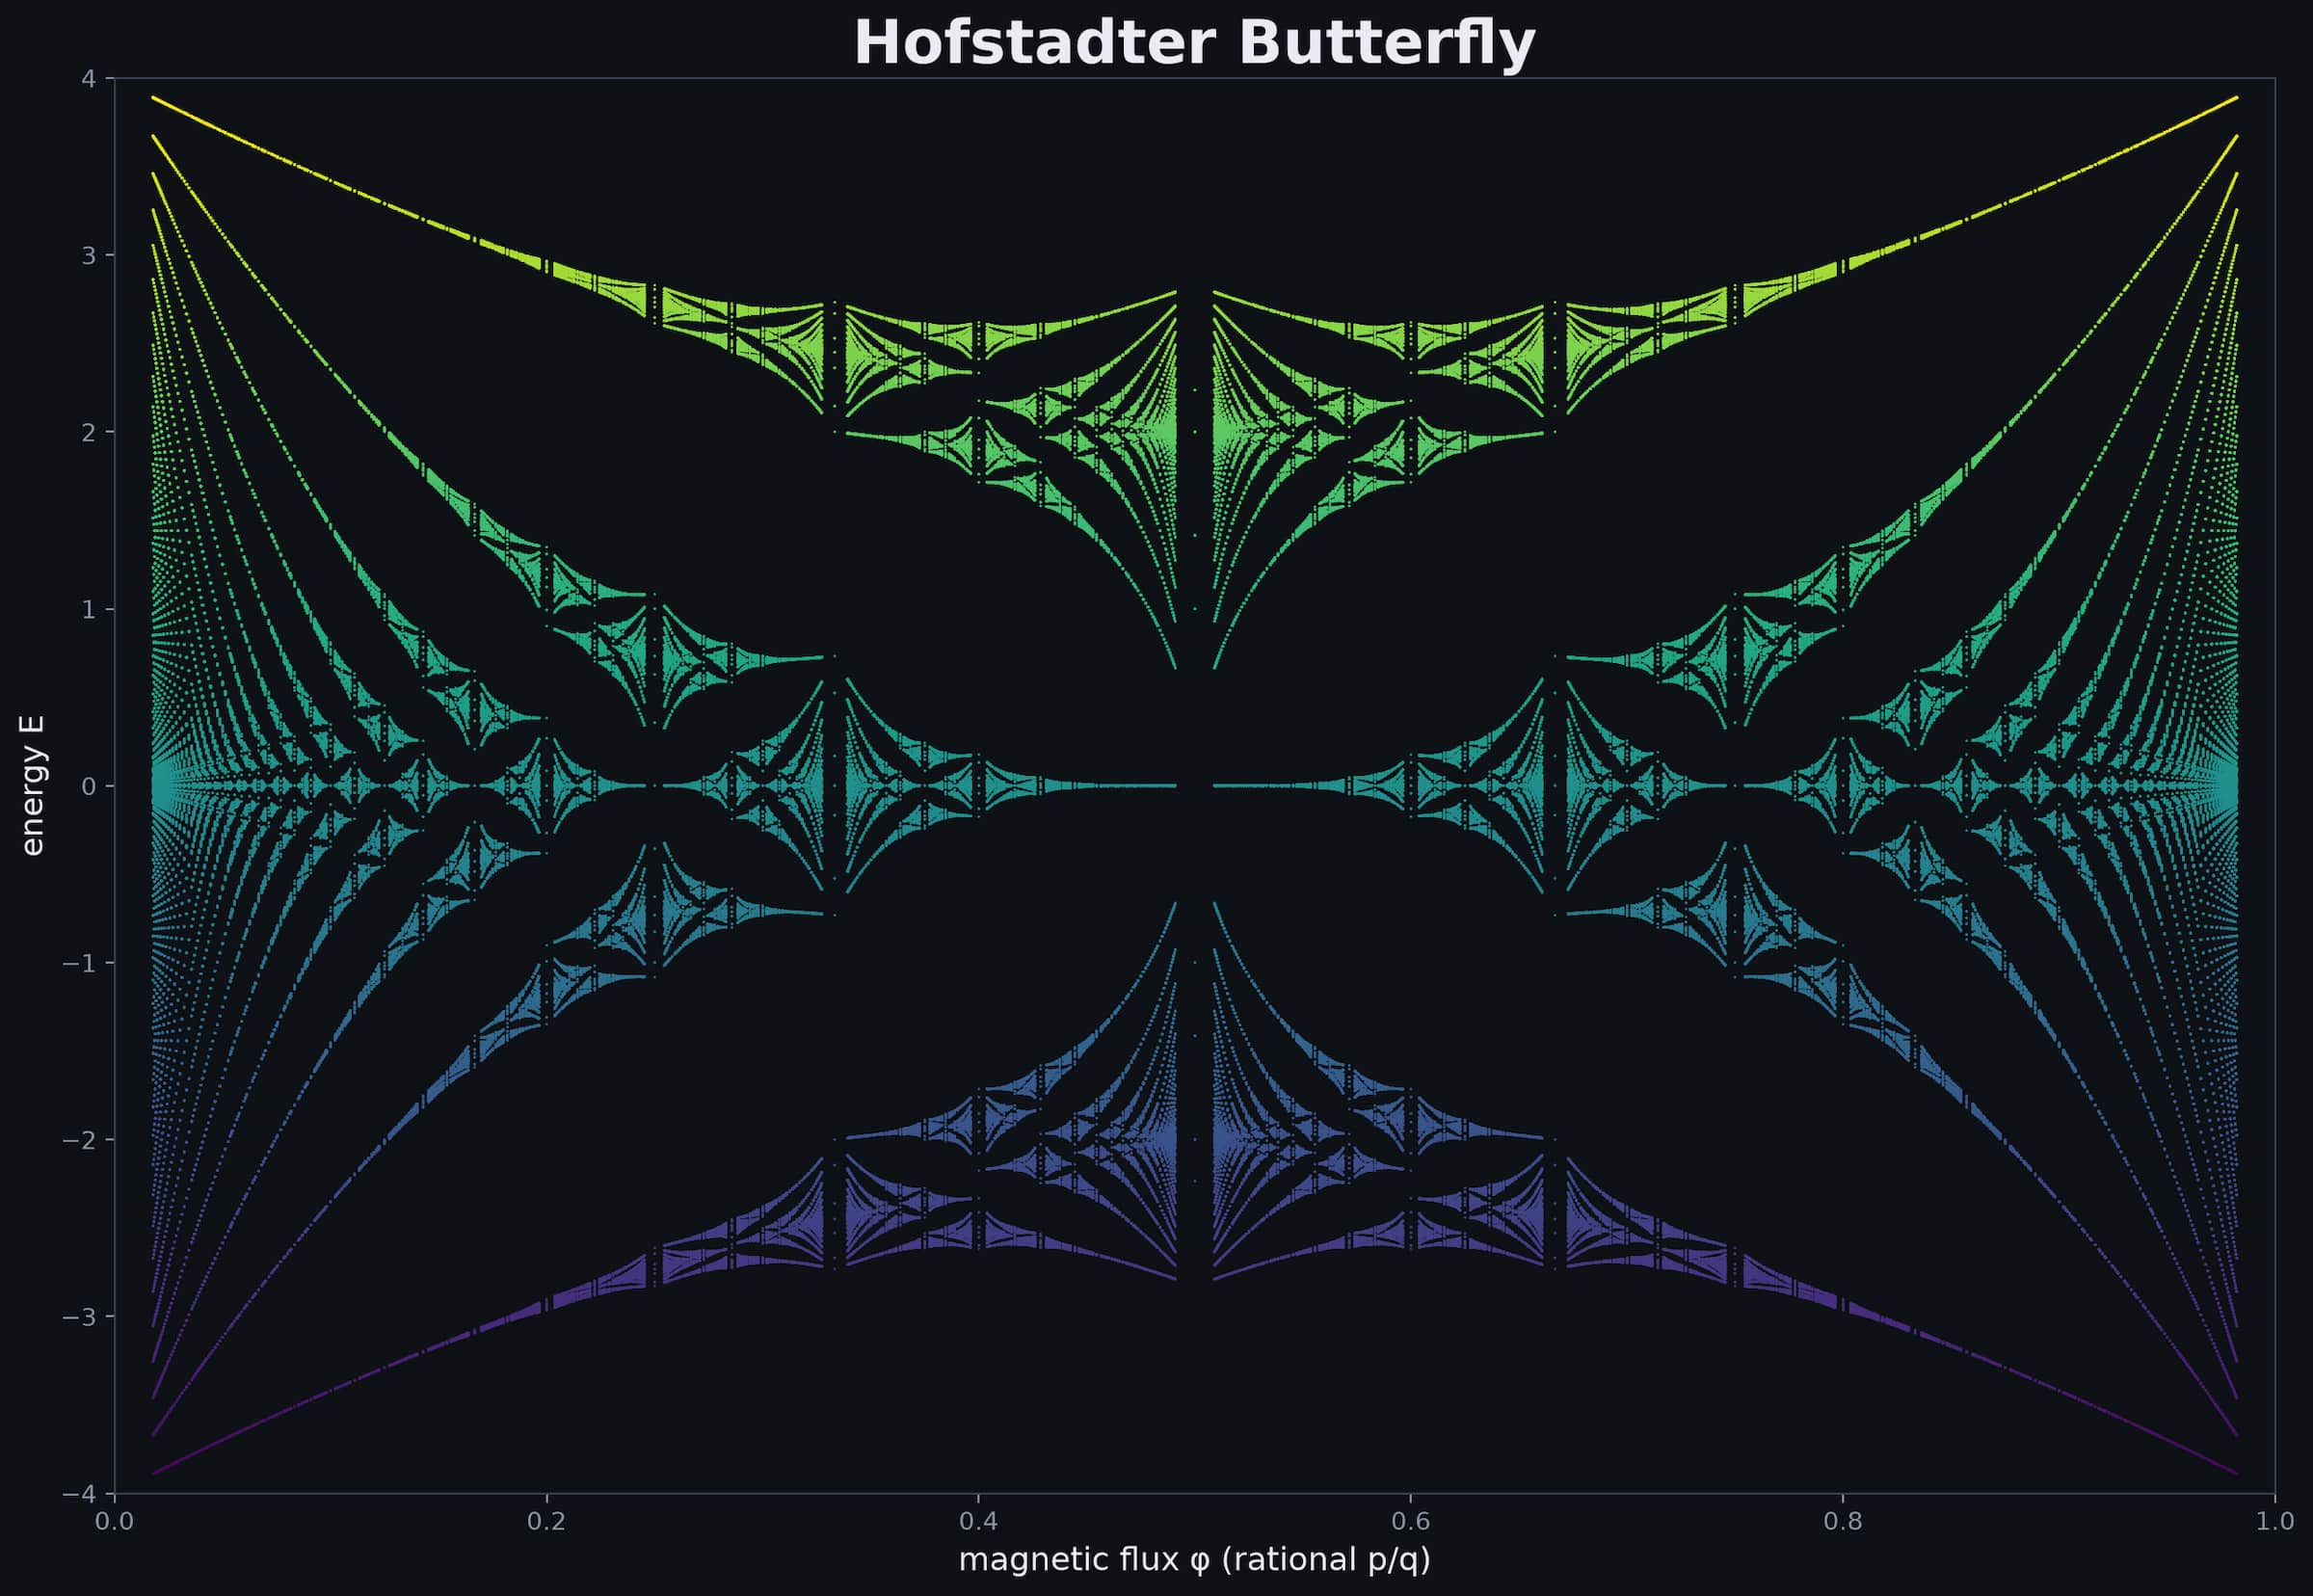
\includegraphics[width=\linewidth]{graphs/hofstadter}
		\caption{}
		\label{fig:supp_a}
		\vspace{0.2cm}
	\end{subfigure}

	\begin{subfigure}{0.62\textwidth}
		\centering
		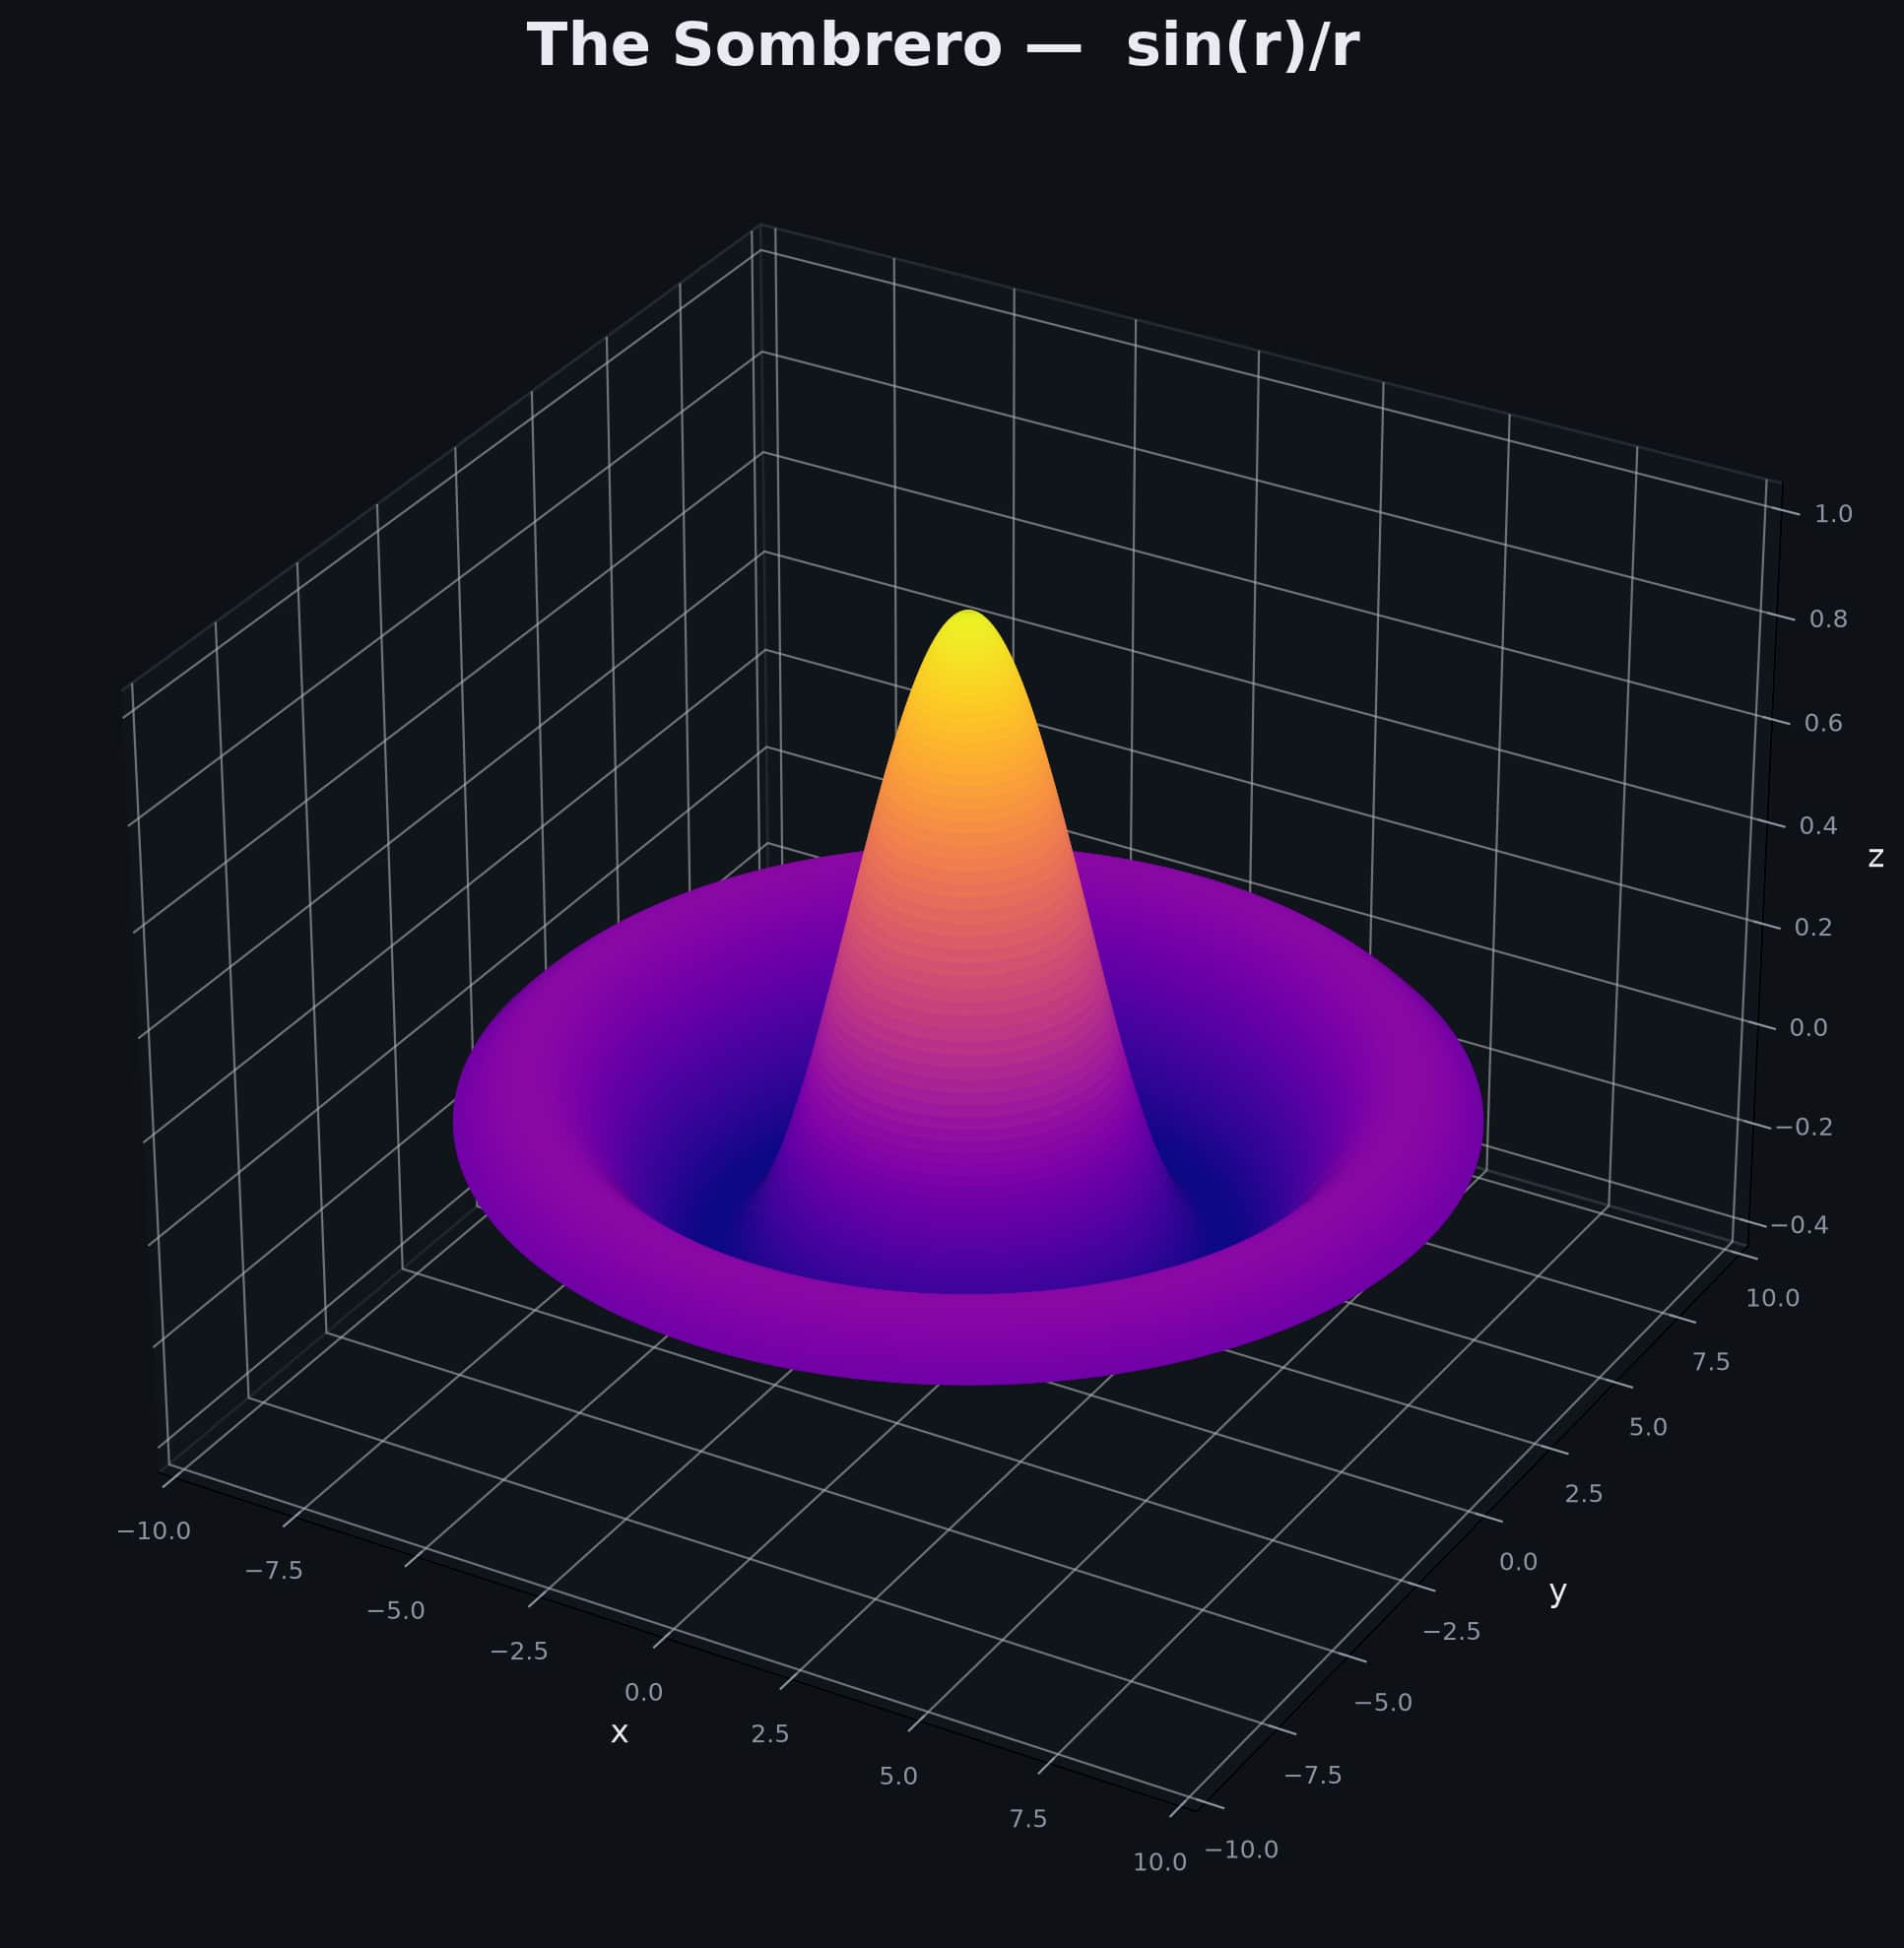
\includegraphics[width=\linewidth]{graphs/sombrero3d}
		\caption{}
		\label{fig:supp_b}
	\end{subfigure}
	\caption{Supplementary results, reproduced at full width. (a) the spectrum
	of a two-dimensional lattice in a magnetic field, plotted against rational
	flux $\varphi = p/q$ \cite{hofstadter1976} — the self-similar structure is
	only visible at this size. (b) the surface of Problem 1 seen from a lower
	viewing angle.}
	\label{fig:supplementary}
\end{figure}

Note the numbering. Because \texttt{main.tex} calls
\verb|\supplementarysection| just before it includes this file,
\cref{fig:supp_a} and \cref{fig:supp_b} carry an \texttt{S} prefix. Figures in
the main text keep their plain numbers.
